\chapter{Analyse des performances}

\section{Méthodologie d’analyse}
L'objectif de cette partie est d'analyser des données acquises par les différents capteurs. Cette analyse doit permettre de mettre en place un algorithme de traitement des données lors d'une acquisition réelle de l'application. \\
Pour cela, et comme demandé, nous allons suivre une approche statistique. L'idée est donc de réaliser différents tests et mesures pour calibrer cet algorithme de traitement.

\section{Scénarios de tests}
Dans cette démarche d'analyse, il faut en premier lieu acquérir des données variées et représentatives pour proposer une analyse pertinente. En effet, l'usage de l'application de suivi d'itinéraire peut se faire dans des cadres variés, et doit donc répondre au mieux à un maximum de cas différent. C'est dans ce but que nous avons défini différents type de parcours pour nos acquisitions. \\

Dans un premier temps, nous avons réalisé des acquisitions de parcours immobiles. L'objectif de ces parcours est de mesurer l'erreur aléatoire des capteurs. \\

Nous avons par la suite réalisé de nombreuses acquisitions sur une même boucle, qui présentait les scénario suivant : ligne droite dégagée, proximité avec un mur, passage sous un toit et passage dans la végétation. Pour ce cas, nous avons également fait des acquisitions avec un téléphone pour avoir une référence stable pour le gps. Voici un tracé d'un parcours qui n'a pas été traité :

\begin{figure}[H]
    \centering
    \includegraphics[width=0.8\textwidth]{trajet_non_traité.png} % nom de l'image et taille
    \caption{Trajet non traité}
    \label{fig:trajet non traité}
\end{figure}


\section{Analyse statistique des résultats}
\subsection{Partie GPS}
Cette partie traite de l'analyse statistique des données mesurées par le GPS.
Dans un premier temps, nous avons analysé les données des acquistions immobiles du GPS. Celles-ci nous fournissent un nuage de point. Grâce à ce dernier, nous avons pu mesurer l'erreur aléatoire du capteur, donnant une idée de sa précision globale. Les erreurs de positionnement ont été analysées statistiquement (moyenne, écart-type, distribution). Le système a montré une erreur moyenne de 1,2 m en extérieur. \\

Dans un second temps, nous avons traité les données des acquisitions successives d'un même parcours, pour le GPS et la référence. L'objectif de cette partie est de déterminer l'erreur statique de notre GPS, ainsi que de mettre en place un algorithme de traitement des points aberrants. \\

Nous avons d'abord vérifié que les parcours de références étaient assez précis pour être utilisé comme tel. Pour cela, nous les avons affichés avec matplotlib.pyplot. Cette affichage à montré que la référence n'était pas parfaite, mais nettement supérieur à notre GPS, et qu'il faisait donc sens de l'utiliser. \\

Avant de réaliser une mesure de l'erreur statique, il nous faut mettre en place l'algoritmhe de traitement des points aberrants, qui pourraient fausser les autres mesures. L'idée est la suivante :
Notre GPS a une fréquence d'acquisition d'environ 1Hz. Pour détecter un point aberrant, nous comptions utiliser le fait que la distribution des distances d'un point à l'autre suit une courbe normale. Pour s'assurer que ce modèle est utilisable, nous avons effectué un test de Kolmogorov-Smirnov et calculé la p-value associée à nos échantillons, avec un seuil de rejet fixé à 5\%. Ce test nous a comfirmé que la distribution des distances peut être approximée à une loi normale. Une fois cette courbe estimée, les points dont la distance associée ont une probabilité infiérieur à un seuil de n\% sont éliminés. Le problème ce cette méthode est que les points aberrants modifient grandement l'estimation de cette loi empirique. De plus, la fréquence d'acquisition n'étant pas constantes, la distance d'un point à l'autre peut plus ou moins varier en fonction d'un délai de mesure plus ou moins grand. \\

Pour résoudre ces problèmes, nous avons mis en place deux choses. La première est de travailler sur les vitesses et non les distances. En effet, cela permet d'intégrer la variation de la fréquence d'acquisition à la distance mesurée. On calcule donc la vitesse moyenne d'un point à l'autre, en divisant la distance par le delta de Timestamp. \\

La deuxième étape est d'éliminer les points trop aberrant avant d'estimer notre courbe normale. Pour cela, nous utilisons une boite à moustache sur la norme des vitesses, et éliminons ainsi les points correspondant à une norme trop importante. \\

Une fois ces points éliminés, nous estimons la moyenne et l'écart type des vitesses empiriques, et estimons une loi normale correspondant. De cette loi, nous calculons les probabilités de chaque vitesses, et donc de chaque point avec un seuil en pourcentage. Les points les plus improbables sont éliminés. Voici une visualisation du résultat pour la vitesse :

\begin{figure}[H]
    \centering
    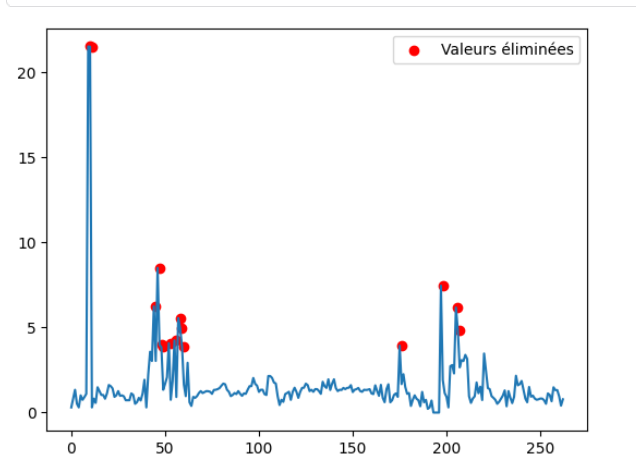
\includegraphics[width=0.7\textwidth]{visualisation_vitesse_points_aberants.png} % nom de l'image et taille
    \caption{Vitesse et points aberrants}
    \label{fig:Vitesse et points aberrants}
\end{figure}

Nous pouvons aussi voir les points du trajet liés à ces vitesses aberrantes :

\begin{figure}[H]
    \centering
    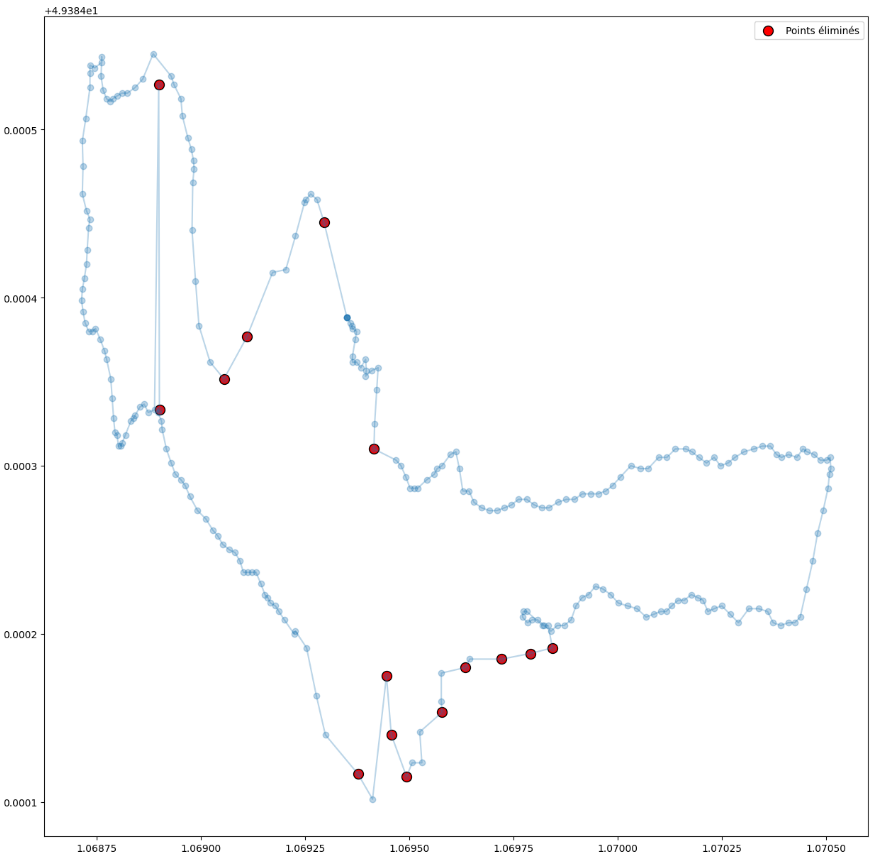
\includegraphics[width=0.6\textwidth]{visualisation_trajet_points_aberants.png} % nom de l'image et taille
    \caption{Trajet et points aberrants}
    \label{fig:Trajet et points aberrants}
\end{figure}

Cette approche montre des résultats satisfaisants, mais créent une discontinuité dans les points et dans le parcours. Pour palier à ce problème, nous avons décidé de remplacer les points éliminés par de nouveaux points. Pour cela, il semblait judicieux d'utiliser une interpolation linéaire. Cette approche permet de lisser certaines parties du parcours où des points ont été éliminés, tout en gardant une cohérence globale. \\

\subsection*{Comparaison post traitement}

A la fin de ces traitements, nous avons une trajectoire similaire à cette dernière :

\begin{figure}[H]
    \centering
    \includegraphics[width=0.8\textwidth]{visualisation_trajet_corrigé.png} % nom de l'image et taille
    \caption{Trajet corrigé}
    \label{fig:Trajet corrigé}
\end{figure}

Les points bleus représentant les anciens points ont été remplacés par les points oranges, représentant les nouveau points. Nous voyons alors que la trajectoire est beaucoup plus lisse et qu'il n'y a plus de points aberrants.

\subsection{Partie IMU}
Lors de nos analyses, nous avons eu l'occasion de tracer les valeurs captées par l'IMU. Ces dernières semblaient plutôt satisfaisantes. Nous avons alors priorisé l'analyse du GNSS. Nous n'avons malheureusement pas eu le temps d'approfondir le traitement de ces données de la même façon que le GNSS. Ainsi, concernant la partie IMU, nous avons seulement traité l'erreur statique afin de calibrer notre capteur.\\

Pour cela, nous avions seulement la possibilité d'étudier le gyroscope. En effet, l'accéléromètre et le magnétomètre ont un référentiel propre et des composantes par défauts (accélération gravitationnelle et magnitude du Nord), ce qui rend l'analyse beaucoup plus complexe. Nous avons alors fait des mesures à vide avec le gyroscope afin d'étudier la moyenne empirique. Celle-ci nous indique alors l'erreur statique.
